\subsection{Continuous functions with compact support}

DEFINITION 1. --- Let X be a topological space, let E be either \(\overline{R}\) or a vector space over R, and let f be a mapping of X into E. The smallest closed set S in X such that \(\mathbf{f}(x)=0\) on X-S (in other words, the closure in X of the set of all \(x\in X\) such that \(\mathbf{f}(x)\neq0\) ) is called the support of f and is denoted Supp(f).

Let X be a locally compact space, E a topological vector space over R or C; recall that \(\mathcal{C}(X;E)\) denotes the vector space of continuous mappings of X into E; when E=R or E=C, we will omit the mention of E in this notation if no confusion can result. We shall denote by \(\mathcal{K}(X;E)\) the subspace of \(\mathcal{C}(X;E)\) formed by the continuous mappings with compact support; for every subset A of X, we denote by \(\mathcal{C}(X,A;E)\) (resp. \(\mathcal{K}(X,A;E)\) ) the subspace of \(\mathcal{C}(X;E)\) (resp. \(\mathcal{K}(X;E)\) ) formed by the mappings f such that Supp(f) ⊂ A. If E=R or E=C, we write \(\mathcal{K}(X)\) (resp. \(\mathcal{K}(X,A)\) ) instead of \(\mathcal{K}(X;\mathbf{R})\) or \(\mathcal{K}(X;\mathbf{C})\) (resp. \(\mathcal{K}(X,A;\mathbf{R})\) or \(\mathcal{K}(X,A;\mathbf{C})\) ), provided no confusion can result; we denote by \(\mathcal{K}_{+}(X)\) the pointed convex cone formed by the functions \(\geqslant0\) of \(\mathcal{K}(X;\mathbf{R})\) .

For every compact subset K of X, the space \(\mathcal{K}(X,K;E)\) may be identified with a subspace of the space of continuous functions \(\mathcal{C}(K;E)\) (namely, the subspace of continuous mappings of K into E that are zero on the boundary \(^{1}\) of K). When \(\mathcal{C}(K;E)\) is equipped with the topology of uniform convergence in K, \(\mathcal{K}(X,K;E)\) is a closed subspace of \(\mathcal{C}(K;E)\) . In particular, if E is a Fréchet space (resp. a Banach space), then so is \(\mathcal{K}(X,K;E)\) , because if the topology of E is defined by the semi-norms \(p_{n}\) (resp. the norm \(x \mapsto \|x\|\) ) then the topology of \(\mathcal{K}(X,K;E)\) is defined by the semi-norms \(\mathbf{f} \mapsto \sup_{x \in K} p_n(\mathbf{f}(x))\) (resp. the norm \(\mathbf{f} \mapsto \sup_{x \in K} \| \mathbf{f}(x) \|\) , denoted \(\| \mathbf{f} \|\) ).

The space \(\mathcal{K}(\mathrm{X};\mathrm{E})\) is the union of the increasing directed family of subspaces \(\mathcal{K}(\mathrm{X},\mathrm{K};\mathrm{E})\) , where K runs over the set of compact subsets of X; moreover, if \(K_{1}\subset K_{2}\) are two compact subsets of X, the canonical injection \(\mathcal{K}(\mathrm{X},\mathrm{K}_{1};\mathrm{E})\to\mathcal{K}(\mathrm{X},\mathrm{K}_{2};\mathrm{E})\) is continuous for the topologies defined above. If E is locally convex, one can therefore define on \(\mathcal{K}(\mathrm{X};\mathrm{E})\) the direct limit \(^{2}\) of the locally convex topologies of the \(\mathcal{K}(\mathrm{X},\mathrm{K};\mathrm{E})\) (TVS, II, §4, No.~4); unless expressly mentioned to the contrary, this will always be the topology in question when we regard \(\mathcal{K}(\mathrm{X};\mathrm{E})\) as a topological vector space.

PROPOSITION 1. --- Let X be a locally compact space, E a Hausdorff locally convex space.

\begin{enumerate}
\def\labelenumi{(\roman{enumi})}
\item
  The locally convex space \(\mathcal{K}(\mathrm{X};\mathrm{E})\) is Hausdorff. For every compact subset \(\mathbf{K}\) of \(\mathbf{X}\) , the topology on \(\mathcal{K}(\mathrm{X},\mathrm{K};\mathrm{E})\) induced by that of \(\mathcal{K}(\mathrm{X};\mathrm{E})\) is the topology of uniform convergence in \(\mathbf{K}\) , and each of the subspaces \(\mathcal{K}(\mathrm{X},\mathrm{K};\mathrm{E})\) is closed in \(\mathcal{K}(\mathrm{X};\mathrm{E})\) .
\item
  If \(\mathbf{E}\) is the product of a finite number of locally convex spaces \(\mathbf{E}_i\) ( \(1 \leqslant i \leqslant n\) ), then the mapping \(f \mapsto (\mathrm{pr}_i \circ f)\) is an isomorphism of the space \(\mathcal{K}(\mathbf{X};\mathbf{E})\) onto the product space \(\prod_{1 \leqslant i \leqslant n} \mathcal{K}(\mathbf{X};\mathbf{E}_i)\) .
\item
  If \(\mathrm{X}\) is the sum of a family \((\mathrm{X}_{\lambda})_{\lambda \in \mathrm{L}}\) of locally compact spaces, then the mapping \(f \mapsto (f|\mathrm{X}_{\lambda})_{\lambda \in \mathrm{L}}\) is an isomorphism of the space \(\mathcal{K}(\mathrm{X};\mathrm{E})\) onto the topological direct sum space of the family \((\mathcal{K}(\mathrm{X}_{\lambda};\mathrm{E}))_{\lambda \in \mathrm{L}}\) .
\item
  Note that, on \(\mathcal{K}(\mathrm{X};\mathrm{E})\) , the topology of uniform convergence in X is compatible with the vector space structure of \(\mathcal{K}(\mathrm{X};\mathrm{E})\) because, for every \(f\in \mathcal{K}(\mathrm{X};\mathrm{E})\) , with (compact) support S, the set \(f(\mathrm{X}) = f(\mathrm{S})\cup \{0\}\) is compact, hence bounded in E (TVS, III, §3, No.~1, Prop. 1). Since this topology \(\mathcal{T}_0\) is locally convex and induces on each \(\mathcal{K}(\mathrm{X},\mathrm{K};\mathrm{E})\) the topology of uniform convergence in K, the same is true of the direct limit topology \(\mathcal{T}\) on \(\mathcal{K}(\mathrm{X};\mathrm{E})\) (TVS, II, §4, No.~4, Remark); moreover, \(\mathcal{T}\) is finer than \(\mathcal{T}_0\) and \(\mathcal{T}_0\) is Hausdorff, therefore \(\mathcal{T}\) is Hausdorff. Finally, suppose that a function \(f\in \mathcal{K}(\mathrm{X};\mathrm{E})\) belongs to the closure of \(\mathcal{K}(\mathrm{X},\mathrm{K};\mathrm{E})\) ; by the definitions, there exists a compact subset \(\mathrm{K}'\supset \mathrm{K}\) of X such that \(f\in \mathcal{K}(\mathrm{X},\mathrm{K}';\mathrm{E})\) . By the foregoing, \(f\) belongs to the closure of \(\mathcal{K}(\mathrm{X},\mathrm{K};\mathrm{E})\) in the space \(\mathcal{K}(\mathrm{X},\mathrm{K}';\mathrm{E})\) , hence belongs to \(\mathcal{K}(\mathrm{X},\mathrm{K};\mathrm{E})\) .
\item
  The criterion for continuity in a direct limit (TVS, II, §4, No.~4, Prop. 5) shows at once that the mapping \(f \mapsto (\mathrm{pr}_i \circ f)\) is continuous and that the same is true of the inverse mapping (for the latter, it suffices to note that if, for every function \(f_i \in \mathcal{K}(\mathrm{X};\mathrm{E}_i)\) , one denotes by \(f_i'\) the mapping of X into E such that \(\mathrm{pr}_i\circ f_i' = f_i\) and \(\mathrm{pr}_j\circ f_i' = 0\) for \(j\neq i\) , then each of the mappings \(f_{i}\mapsto f_{i}^{\prime}\) is continuous).
\item
  Each compact subset \(\mathbf{K}\) of \(\mathbf{X}\) intersects only the \(\mathbf{X}_{\lambda}\) of a finite subfamily \((\mathbf{X}_{\lambda})_{\lambda \in \mathbf{H}}\) of \((\mathbf{X}_{\lambda})_{\lambda \in \mathbf{L}}\) , and it is immediate that if one sets \(\mathrm{K}_{\lambda} = \mathrm{K} \cap \mathrm{X}_{\lambda}\) for \(\lambda \in \mathbf{H}\) , the mapping \(f \mapsto (f|\mathrm{X}_{\lambda})_{\lambda \in \mathbf{H}}\) is an isomorphism of \(\mathcal{K}(\mathrm{X},\mathrm{K};\mathrm{E})\) onto \(\prod_{\lambda \in \mathbf{H}} \mathcal{K}(\mathrm{X}_{\lambda},\mathrm{K}_{\lambda};\mathrm{E})\) . Conversely, for every function \(f_{\lambda} \in \mathcal{K}(\mathrm{X}_{\lambda};\mathrm{E})\) , let \(f_{\lambda}^{\prime \prime}\) be the mapping of \(\mathbf{X}\) into \(\mathbf{E}\) such that \(f_{\lambda}^{\prime \prime}|\mathrm{X}_{\lambda} = f_{\lambda}\) and \(f_{\lambda}^{\prime \prime}|\mathrm{X}_{\mu} = 0\) for \(\mu \neq \lambda\) ; it is immediate that the mapping \(f_{\lambda} \mapsto f_{\lambda}^{\prime \prime}\) of \(\mathcal{K}(\mathrm{X}_{\lambda};\mathrm{E})\) into \(\mathcal{K}(\mathrm{X};\mathrm{E})\) is continuous. The assertion (iii) follows from these remarks and the criterion for continuity in direct limits (TVS, II, §4, No.~4, Prop. 5).
\end{enumerate}

PROPOSITION 2. --- Let X be a locally compact space, E a Hausdorff locally convex space.

\begin{enumerate}
\def\labelenumi{(\roman{enumi})}
\item
  If \(\mathbf{E}\) is a Fréchet space, then the space \(\mathcal{K}(\mathbf{X};\mathbf{E})\) is barreled.
\item
  If X is paracompact then, for every bounded set B in \(\mathcal{K}(\mathrm{X};\mathrm{E})\) , there exists a compact subset K of X such that \(\mathrm{B}\subset \mathcal{K}(\mathrm{X},\mathrm{K};\mathrm{E})\) .
\end{enumerate}

Suppose E is a Fréchet space. Then, for every compact subset K of X, \(\mathcal{K}(X,K;E)\) is a Fréchet space, hence is barreled, and one knows that a direct limit of barreled spaces is barreled (TVS, III, §4, No.~1, Cor. 3 of Prop. 3), whence (i).

If X is paracompact, one knows (GT, I, §9, No.~10, Th. 5) that X is the sum of a family \((\mathrm{X}_{\lambda})_{\lambda \in \mathrm{L}}\) of locally compact spaces that are countable at infinity; \(^{3}\) thus (Prop. 1, (iii)), \(\mathcal{K}(\mathrm{X};\mathrm{E})\) is the topological direct sum of the family of subspaces \(\mathcal{K}(\mathrm{X}_{\lambda};\mathrm{E})\) ( \(\lambda \in L\) ). By virtue of the characterization of the bounded sets in a topological direct sum (TVS, III, §1, No.~4, Prop. 5), every bounded set in \(\mathcal{K}(\mathrm{X};\mathrm{E})\) is contained in the sum of a finite number of subspaces \(\mathcal{K}(\mathrm{X}_{\lambda};\mathrm{E})\) , and it will suffice to prove that every bounded set in \(\mathcal{K}(\mathrm{X}_{\lambda};\mathrm{E})\) is contained in a subspace \(\mathcal{K}(\mathrm{X}_{\lambda},\mathrm{K}_{\lambda};\mathrm{E})\) , with \(K_{\lambda}\) compact in \(X_{\lambda}\) . We are thus reduced to the case that X is countable at infinity, in other words is the union of a sequence of relatively compact open sets \(U_{n}\) such that \(\overline{U}_{n} \subset U_{n+1}\) (GT, I, §9, No.~9, Prop. 15). But then \(\mathcal{K}(\mathrm{X};\mathrm{E})\) is the strict direct limit of the sequence of spaces \(\mathcal{K}(\mathrm{X},\overline{\mathrm{U}}_{n};\mathrm{E})\) , whence the assertion (ii) (TVS, III, §1, No.~4, Prop. 6).

We shall say that a subset H of \(\mathcal{K}(X;E)\) is strictly compact if it is compact and if there exists a compact subset K of X such that \(H \subset \mathcal{K}(X,K;E)\) . It follows at once from Proposition 2 that if X is a paracompact locally compact space and if E is Hausdorff, then every compact set in \(\mathcal{K}(X;E)\) is strictly compact. One can give examples of locally compact spaces X (not paracompact) such that there exist sets in \(\mathcal{K}(\mathrm{X};\mathbf{R})\) that are compact but not strictly compact (Exercises 3 and 4).

\pandocbounded{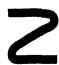
\includegraphics[keepaspectratio]{images/part001_73a6a0da.jpg}}

We recall that, by virtue of Ascoli's theorem (GT, X, §2, No.~5, Cor. 3 of Th. 2), a strictly compact subset H of \(\mathcal{K}(\mathrm{X};\mathrm{E})\) contained in \(\mathcal{K}(\mathrm{X},\mathrm{K};\mathrm{E})\) is characterized by the following conditions: \(1^{\circ}\) it is closed; \(2^{\circ}\) it is equicontinuous; \(3^{\circ}\) for every \(x\in \mathbf{K}\) , the set \(\mathrm{H}(x)\) is relatively compact in E.

COROLLARY. --- Let X be a paracompact, locally compact space; if E is a quasi-complete locally convex space, then the space \(\mathcal{K}(X;E)\) is quasi-complete.

It suffices, by virtue of Proposition 2, (ii), to note that for every compact subset K of X, \(\mathcal{K}(X,K;E)\) is a closed subspace of \(\mathcal{C}(K;E)\) , which is quasi-complete since every bounded subset of \(\mathcal{C}(K;E)\) consists of functions taking values in a same bounded subset of E.

